%!TEX root = ../main.tex
\chapter{Schätzer}
\section{Allgemeines zum Schätzen}
Beim Schätzen wollen wir von einer Beobachtung einer (teilweise) unbekannten Verteilung auf Parameter der Verteilung schließen.

Das kann zum einen bedeuten, dass man versucht aus einer Stichprobe zu folgern, um welche Art von Verteilung es sich handelt. Ebenso kann man Parameter einer bekannten Verteilung schätzen.

Man sieht sofort dass man beim Schätzen einige Angaben entweder wissen oder Annahmen treffen muss.
Selbstverständlich kann man nur Parameter einer Verteilung schätzen wenn man annimmt dass sich beim zugrundeliegenden Experiment um diese Verteilung handelt.

Es gibt verschiede Arten zu Schätzen, so kann man einerseits einen Bereich angeben in dem sich der Parameter mit einer gewissen Sicherheit befindet (Intervallschätzer). Andererseits kann man auch einen Wert angeben den der Parameter bei gegebener Stichprobe am wahrscheinlichsten annimmt (Punktschätzer).











\section{Punktschätzer}
Punktschätzer liefern einen genauen Wert als Ergebnis des Schätzens. Dabei ist dieser Wert der, der bei gegebener Stichprobe am wahrscheinlichsten ist.



\paragraph{Unspezifische Parameter}
Es wird zwischen zwei Arten der Schätzparameter unterschieden, unspezifische Parameter die keine Informationen über das Experiment beinhalten. So sind die folgenden zum Beispiel unspezifische Parameter
\begin{itemize}
	\item Erwartungswert $E(X)$ oder Varianz $V(X)$,
	\item der Median oder andere Quantile einer Zufallsvariable,
	\item die Korrelation von zwei Zufallsvariablen.
\end{itemize}
\paragraph{Spezifische Parameter}
Dagegen enthalten spezifische Parameter Informationen auch über das konkrete Experiment. Einige Beispiele hierfür wären
\begin{itemize}
	\item Der Parameter $p$ der Binomialverteilung $\binomial(n,p)$,
	\item $\sigma^2,\mu$ einer Normalverteilung $\norm(n,p)$,
	\item oder $\lambda$ von $\poisson(\lambda)$.
\end{itemize}
Um diese Parameter zu schätzen benötigt man eine sogenannte Schätzstatistik. 

\begin{definition}{Schätzstatistik}
	Eine Schätzstatistik oder Schätzfunktion ist eine Abbildung
	\begin{equation*}
		g(X_1,\ldots,X_n)
	\end{equation*}
	in den Stichprobenvariablen $X_i$.
	Für eine Stichprobe $\omega$ (Realisierung) $x_1,\ldots,x_n$ heißt der Wert
	\begin{equation*}
		g(x_1,\ldots,x_n)=g(X_1(\omega),\ldots,X_n(\omega))
	\end{equation*}
	Schätzwert der Realisierung.
\end{definition}
\paragraph{Beispiele:}
Die folgenden Zufallsvariablen sind Schätzstatistiken
\begin{equation}\label{eq:schatzstatistiken}
	\begin{split}
		\overline X=g(X_1,\ldots,X_n)&\coloneqq \frac1n\sum_{i=1}^n X_i&&\text{für }\mu=E(X)\\
		S^2 =g(X_1,\ldots,X_n)&\coloneqq \frac{1}{n-1}\sum_{i=1}^n (X_i-\overline X)^2&&\text{für }\sigma^2=V(X)\\
		\quad \tilde S^2 =g(X_1,\ldots,X_n)&\coloneqq\frac1n\sum_{i=1}^n (X_i-\overline X)^2&&\text{für }\sigma^2=V(X)
	\end{split}
\end{equation}


Betrachtet man Schätzstatistiken, stellt sich die Frage ob diese tendenziell den richtigen Wert liefern. Diese Eigenschaft nennt man Erwartungstreue.

\begin{definition}{Erwartungstreue}
	Man nennt eine Schätzstatistik $g(X_1,\ldots,X_n)$ für den Parameter $\alpha$ \emph{erwartungstreu}, falls
	\begin{equation*}
		E_\alpha(g(X_1,\ldots,X_n))=\alpha.
	\end{equation*}
	
	Gilt lediglich, dass
	\begin{equation*}
		\lim_{n\to\infty} E_\alpha(g(X_1,\ldots,X_n))=\alpha
	\end{equation*}
	so nennt man $g$ \emph{asymptotisch erwartungstreu}.

	Allgemein ist die \emph{Verzerrung} oder der \emph{Bias}
	\begin{equation*}
		\operatorname{Bias}_\alpha (g(X_1,\ldots,X_n))=E_\alpha(g(X_1,\ldots,X_n))-\alpha
	\end{equation*}
\end{definition}
Untersuchen wir nun die Schätzstatistiken aus \autoref{eq:schatzstatistiken} auf Erwartungstreue.

Wir sehen aus
\begin{equation*}
	E_\mu(\overline X)=E_\mu\left( \frac1n\sum_{i=1}^n X_i \right)=\frac1n\sum_{i=1}^n E_\mu(X_i)=\mu,
\end{equation*}
dass $\overline X$ erwartungstreu ist.

Für $S^2$ und $\tilde S^2$ betrachten wir zunächst die folgende Umformung
\begin{align*}
	E_{\sigma^2}(S^2)&=E_{\sigma^2}\left( \frac{1}{n-1}\sum_{i=1}^n (X_i-\overline X)^2 \right)\\
	&=\frac{1}{n-1} * E_{\sigma^2}\left( \sum_{i=1}^n (X_i-\overline X)^2 \right)\\
	&=\frac{1}{n-1} * E_{\sigma^2}\left( \sum_{i=1}^n X_i^2- 2\overline X X_i +\overline X^2 \right)\\
	&=\frac{1}{n-1} * E_{\sigma^2}\left( \sum_{i=1}^n X_i^2- 2\overline X n\overline X +n\overline X^2 \right)\\
	&=\frac{1}{n-1} * E_{\sigma^2}\left( \sum_{i=1}^n X_i^2- n\overline X \right)\\
	&=\frac{1}{n-1} * \left(\sum_{i=1}^n E_{\sigma^2}(  X_i^2 )- n E_{\sigma^2}(\overline X ) \right)\\
	\intertext{Mit dem Verschiebungssatz $V(Z)=E(Z^2)-E(Z)^2$ folgt daraus nun, dass $E(X_i^2)=V(X_i)+E(X_i)^2=\sigma^2+\mu^2$ und analog $E(\overline X^2)=V(\overline X)+E(\overline X)^2=\frac{\sigma^2}{n}+\mu^2$. Damit ergibt sich}
	E_{\sigma^2}(S^2)&=\frac{1}{n-1} \left(\sum_{i=1}^n (\sigma^2+\mu^2)-n\left(\frac{\sigma^2}{n}+\mu^2\right)\right)\\
	&=\frac{1}{n-1} \left(n\sigma^2+n\mu^2-(\sigma^2+n\mu^2)\right) \\
	&=\frac{1}{n-1} (n-1)*\sigma^2
\end{align*}
Man sieht sofort, dass $S^2$ ein erwartungstreuer Schätzer für $\sigma^2$ während $\tilde S^2$ nicht erwartungstreu ist. Allerdings $\tilde S^2$ ist asymptotisch erwartungstreu
\begin{equation*}
 	\lim_{n\to\infty} E_{\sigma^2}(\tilde S^2)=\lim_{n\to\infty} \sigma^2-\frac{\sigma^2}n=\sigma^2
\end{equation*} 

Hiervon ausgehend ist die Abweichung einer erwartungstreuen Schätzstatistik interessant.
\begin{definition}{Standardfehler für erwartungstreue Schätzstatistiken}
	Der Standardfehler einer erwartungstreuen Schätzstatistik $g$ ist definiert als der Wert%
	\begin{equation*}
		\sigma_g = \sqrt{V(g(X_1,\ldots,X_n))}
	\end{equation*}
\end{definition}
\paragraph{Beispiel:}
Der Standardfehler von $\overline X$ ist
\begin{equation*}
	\sigma_g = \sqrt{V(\overline X)}= \sqrt{\frac{\sigma^2}{n}}=\frac\sigma {\sqrt n}
\end{equation*}
So wird ein weiteres Problem klar - $\sigma^2$ ist möglicherweise unbekannt und muss ebenfalls geschätzt werden.



\subsection{Maximum-Likelihood-Schätzer}
Die Maximum-Likelihood-Schätzmethode verwendet eine sogenannte Likelihoodfunktion $L$. Diese ist abhängig vom zu schätzenden Parameter $\alpha$, man sucht dann den Wert für $\alpha$ so, dass $L(\alpha)$ ein Maximum annimmt. Häufig wird dieser Wert mit einem Dach gekennzeichnet. 

Das Ergebnis dieses Schätzers wäre also allgemein
\begin{equation*}
	\hat\alpha = \underset\alpha\argmax L(\alpha)
\end{equation*}

Hierbei hängt die Likelihoodfunktion davon ab, was bei welcher Verteilung geschätzt wird. 


Wir wollen den Maximum-Likelihood-Schätzer anhand der Binomialverteilung betrachten.
Hierbei macht nur Schätzen des Parameters $p$ Sinn, denn selbst wenn nur eine einzige Stichprobe vorliegt, sieht man sofort welchen Wert $n$ hat.

Es liegt also eine Verteilung 
\begin{equation*}
	X\sim\binomial(n,p)
\end{equation*}
zugrunde, hierbei ist $n$ bekannt und fest, $p\in(0,1)$ wollen wir herausfinden.

Liegt uns nun eine Stichprobe $\omega$ vor, so ist auch $X(\omega)=k$ bekannt als die Anzahl Treffer in den $n$ Bernoulli-Experimenten.

Zum Schätzen fehlt uns noch die Likelihoodfunktion, diese ist hier
\begin{equation*}
	L:(0,1)\rightarrow[0,1], \enspace L(p)=P_p(X=k)=\binom{n}{k}*p^k(1-p)^{n-k}
\end{equation*}

Das heißt, es ist die Wahrscheinlichkeit dass $X$ mit Trefferwahrscheinlichkeit $p$ (als Parameter!) den Wert $k$ annimmt. Man sieht, dass diese Funktion ihr Maximum bei dem Wert für $p$ annimmt, unter dem es am wahrscheinlichsten ist, die Stichprobe $\omega$ zu erhalten.
\begin{center}
	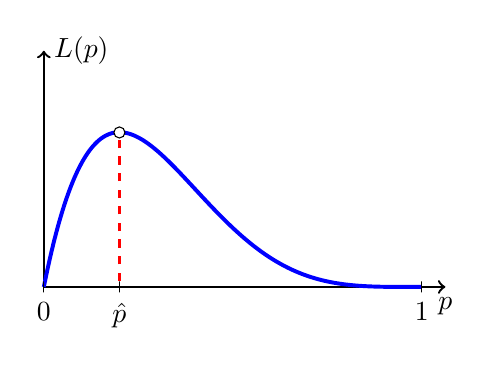
\begin{tikzpicture}[scale=0.6]
		\draw[->, line width=0.3mm] (0,0) to (8.5,0) node[below] {$p$};
		\draw[->, line width=0.3mm] (0,0) to (0,5) node[right] {$L(p)$};

		\draw[line width=0.5mm,scale=8,domain=0:1,smooth,variable=\x,blue, samples=100] plot ({\x},{5*\x * ((1-\x)^(4))});


		%\draw[line width=0.5mm,scale=8,domain=0.001:1,smooth,variable=\x,green, samples=100] plot ({\x},{0.15*(5*(1-\x)^4-20*\x*(1-\x)^3)});	

		\draw (1.6,0) node (hatp) [rectangle,inner sep = 0pt,minimum size = 0pt,minimum height=4pt,draw, label={below:$\hat p$}] {};
		\draw (1.6,3.27) node (Lhatp) [fill = white,circle,inner sep = 0pt,minimum size = 4pt,draw] {};

		
		\draw (0,0) node (null) [rectangle,inner sep = 0pt,minimum size = 0pt,minimum height=4pt,draw, label={below:$0$}] {};
		\draw (8,0) node (eins) [rectangle,inner sep = 0pt,minimum size = 0pt,minimum height=4pt,draw, label={below:$1$}] {};
		

		\draw[red, line width=0.3mm, dashed] (hatp) -- (Lhatp);
			
	\end{tikzpicture}	
\end{center}
Den Wert $\hat p$ zu berechnen würde hier durch Ableiten und anschließendem Bestimmen der Nullstelle erfolgen
\begin{equation*}
	\frac{\diff}{\diff p}L(\hat p)\overset!= 0.
\end{equation*}

\paragraph{Beispiel:}
Wir wollen dies nun nochmal an einem Beispiel veranschaulichen. Wir schätzen wiederum $p$ einer Binomialverteilung, schließen damit später aber auf einen anderen Wert.
\begin{eBox}{}{}
	Um die Populationsgröße $N$ einer Fischart in einem See zu schätzen, gehen wir folgendermaßen vor: Wir markieren von dieser Art $m=50$ Fische in einem See, fangen später $n=200$ Stück und stellen fest, dass $k=16$ davon markiert sind.

	Wir nehmen an, dass das Untersuchen der Stichprobe auf Markierungen eine Folge von $n$ unabhängigen Bernoulli-Experimenten mit Trefferwahrscheinlichkeit $p=\frac mN$ ist. Also beschreibt $p$ den Anteil der markierten Fische im See.
\end{eBox}
Wir verwenden die zuvor besprochene Likelihoodfunktion $L(p)$, denn mit $p=\frac mN$ können wir auf $N$ schließen. 

Sei $X$ eine Zufallsvariable die die Anzahl markierter Fische in der Stichprobe beschreibt, damit ist $X \sim \binomial(200,p)$ verteilt. 

Die Likelihoodfunktion ist mit diesen Werten
\begin{equation*}
	L(p)=P_p(X=k)=\binom{200}{k}* p^{k}(1-p)^{200-k}
\end{equation*}
Damit folgt
\begin{align*}
	\frac{\diff}{\diff p}L(p) &= \binom{200}{k}*\left[ k*p^{k-1}(1-p)^{200-k} - p^k*(200-k)*(1-p)^{200-k-1}\right]\\
	&=\underbrace{\binom{200}{16}* p^{k-1}(1-p)^{200-k-1}}_{>0} * \left[ k(1-p)-200p+kp \right]\\
\end{align*}%
Da wir uns für Nullstellen interessieren, betrachten wir nur noch den rechten Teil und erhalten
\begin{align*}
	k(1-\hat p)-200\hat p+k\hat p&\overset != 0\\
	k-k\hat p-200\hat p+k\hat p &= 0\\
	k-200\hat p&=0
\end{align*}
Für unsere Stichprobe $\omega$ ist $X(\omega)=k=16$, damit ist
\begin{align*}
	\hat p =\frac{m}{N} =\frac k{200}\Rightarrow N&=\frac {m*200}{k}\\
	\Rightarrow N &= \frac{50*200}{16} = 625
\end{align*}

Wir haben damit die Populationsgröße der Fischart auf 625 geschätzt.



\subsection{Bayes-Schätzer}
Wir betrachten die Zufallsvariable $X$ mit dem zugehörigen Wahrscheinlichkeitsraum $(X(\Omega), P_\theta)$. Hierbei wollen wir den Parameter $\theta$ schätzen. 

Der Bayes-Schätzer stellt eine komplett andere Herangehensweise an das Schätzen dar, hier wird der gesuchte Parameter als eine Zufallsvariable aufgefasst. So können weitere Annahmen wie Erfahrung aus anderen Experimenten oder ein grobes Vorwissen über den Sachverhalt in den Schätzvorgang eingehen.

Achtung, die Werte der Zufallsvariable $\theta$ werden ebenfalls $\theta$ genannt.
\begin{enumerate}
	\item 
	Wir betrachten also zunächst die gemeinsame Dichte $f(x,\theta)$ wobei $x\in X(\Omega)$ und $\theta\in \Theta\subseteq[0,1]$. 

	Der einfachere Fall ist hierbei, wenn es sich sowohl bei $X$ als auch $\theta$ um diskrete Zufallsvariablen handelt (wir betrachten nur diesen), dann kann man die gemeinsame Verteilung durch die Kontingenztafel darstellen
	$$
	\begin{array}{|c|cccc|c|}
		\hline \text{gem. Dichte}&x_1&x_2&x_i&x_m&\\\hline
		\theta_1&f(x_1,\theta_1)&f(x_2,\theta_1)&\cdots&f(x_m,\theta_1)&\\
		\theta_2&f(x_1,\theta_2)&\ddots&&&\\
		\vdots&\vdots&&f(x_i,\theta_j)&\vdots&f(\theta_j)=\sum_{i=1}^m f(x_i,\theta_j)\\
		\theta_n&f(x_1,\theta_n)&\cdots&&f(x_m,\theta_n)&\\\hline
		\text{Randdichte}&&&f(x_j)=\sum_{j=1}^n f(x_i,\theta_j)&&\\\hline
	\end{array}
	$$

	\item Nun kann man die bedingte Verteilung von $X$ unter gegebenem $\theta$ darstellen als
	\begin{equation*}
		f(x_i|\theta_j)=P_\theta(X=x_i)
	\end{equation*}
	Da hierbei $\theta$ nun fest gewählt ist, kann man dies problemlos berechnen.

	\item Jetzt kommt der Punkt an dem die Besonderheit der Bayes-Schätzung eingeht, man legt eine sogenannte \emph{a-priori-Dichte} für $\theta$ fest. 
	Zum Beispiel kann dies eine Gleichverteilung auf ganz $\Theta$ sein, das würde bedeuten, man hat kein besonderes Vorwissen über $\theta$.
	Man kann aber genaso vorgeben, dass einige Werte für $\theta$ wahrscheinlicher als andere sind, dies beeinflusst das Ergebnis und kann so zu genaueren Schätzergebnissen führen.

	\item Als letztes berechnet man noch die Randdichte von $X$, unabhängig vom Parameter $\theta$
	\begin{align*}
		f(x_j)&=P(X=x_j)=\sum_{i=1}^n f(x_j|\theta_i)*f(\theta_i)\quad\text{(Satz v. d. totalen Wahrscheinlichkeit)}\\
		&=\sum_{i=1}^n f(x_j,\theta_i)
	\end{align*}
\end{enumerate}

Jetzt führen wir ein Experiment durch. Liegt uns nun eine Stichprobe $\tilde x\in\simpleset{x_1,\ldots,x_m}$ vor, so können wir damit von der a-priori-Dichte auf die sogenannte a-posteriori-Dichte $f(\theta_i|\tilde x)$ schließen.
Wir erhalten also eine Aussage über die Wahrscheinlichkeit eines $\theta_i$ bei gegebenem Ergebnis $\tilde x$.
\begin{align*}
	f(\theta_i|\tilde x)&=\frac{f(\tilde x|\theta_i)*f(\theta_i)}{f(\tilde x)}\quad\text{(Satz von Bayes)}\\
	&=\frac{f(\tilde x,\theta_i)}{\sum_{k=1}^m f(\tilde x|\theta_k) * f(\theta_k)}
\end{align*}

Hiervon ausgehend gibt es zwei Arten, sich auf ein $\theta$ festzulegen.
\paragraph{A-posteriori-Erwartungswert}
Die erste Variante ist, das Schätzergebnis als den Erwartungswert
\begin{equation*}
	\hat\theta_p = E(\theta|\tilde x) = \sum_{i=1}^n \theta_i*f(\theta_i|\tilde x)
\end{equation*}
zu wählen. (Beziehungsweise das nächstgelegene $\theta\in\Theta$.)

\paragraph{Maximum-a-posteriori-Schätzer}
Analog zum Maximum-Likelihood-Schätzer kann man das Maximum der a-posteriori-Dichte als Schätzergebnis wählen
\begin{equation*}
	\hat\theta_{\text{MAP}} = \underset\theta\argmax f(\theta|\tilde x).
\end{equation*}

Führt man den Bayes-Schätzer ohne Vorwissen - d.h. gleichverteiltes $\theta$ - durch, so stimmt $\hat\theta_{\text{MAP}}$ mit dem Maximum-Likelihood-Schätzer überein.



\subsection{Kleinste Quadrate-Schätzer}
Der kleinste Quadrate-Schätzer minimiert die Summe der quadratischen Abweichungen.

So eignet er sich zum Beispiel zum Schätzen des Erwartungswerts $\mu$,
\begin{align*}
	Q(\mu) &= \sum_{i=1}^n(X_i-\mu)^2\\
	\intertext{dabei wird das arithmetische Mittel als Schätzstatistik verwendet}
	\frac{\diff}{\diff \mu} Q(\mu)&= -2\sum_{i=1}^n(X_i-\mu)\overset != 0\\
	\Rightarrow \quad \hat\mu&= \frac1n \sum_{i=1}^n X_i = \overline X.
\end{align*}


